\documentclass[tikz,border=2pt]{standalone}
\usepackage{amsmath,amssymb}
\usepackage{pgfplots}
\pgfplotsset{compat=1.18}
\usetikzlibrary{arrows.meta}
\begin{document}
% M/G/1 station of Exercise 6.4.6 with availability held at A = 6/7: lambda = 4, S_0 = 1/6 deterministic,
% exponential repairs, lambda_f = 1/(6 E[R]). Then rho = 7/9, C_s^2 = (72/49) E[R] and the
% Pollaczek-Khinchine/Sakasegawa value is E[W] = 49/144 + E[R]/2 (hours); E[R] = 1/2 gives 85/144.
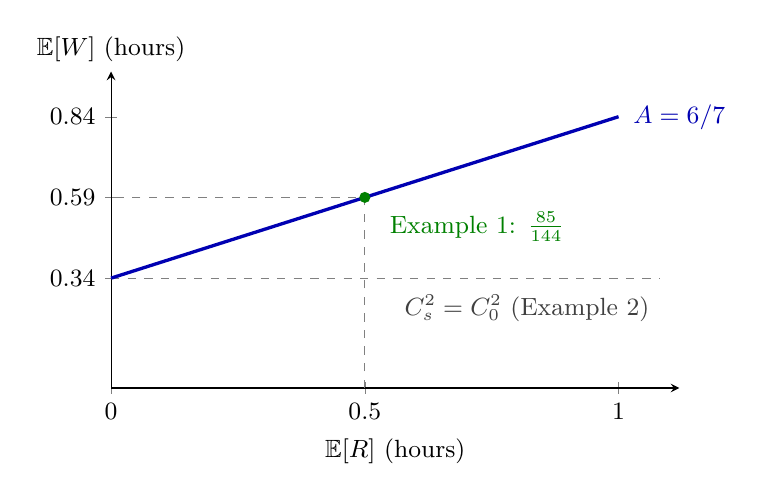
\begin{tikzpicture}[font=\small, >={Latex[length=2mm]}]
  \begin{axis}[
    axis lines=left, xmin=0, xmax=1.12, ymin=0, ymax=0.98,
    xtick={0,0.5,1}, ytick={0.34,0.59,0.84},
    yticklabels={$0.34$,$0.59$,$0.84$},
    xlabel={$\mathbb{E}[R]$ (hours)}, ylabel={$\mathbb{E}[W]$ (hours)},
    xlabel style={at={(axis description cs:0.5,-0.13)}, anchor=north},
    ylabel style={rotate=-90, at={(axis description cs:0,1)}, anchor=south},
    width=8.8cm, height=5.6cm, clip=false]
    \draw[gray, thin, dashed] (axis cs:0,0.3403) -- (axis cs:1.08,0.3403);
    \node[gray!50!black, anchor=north east] at (axis cs:1.08,0.32) {$C_s^2=C_0^2$ (Example 2)};
    \addplot[blue!70!black, very thick, domain=0:1, samples=2] {49/144 + x/2};
    \node[blue!70!black, anchor=west] at (axis cs:1.01,0.84) {$A=6/7$};
    \draw[gray, thin, dashed] (axis cs:0.5,0) -- (axis cs:0.5,0.5903) -- (axis cs:0,0.5903);
    \fill[green!50!black] (axis cs:0.5,0.5903) circle (2pt);
    \node[green!50!black, anchor=north west] at (axis cs:0.53,0.575) {Example 1: $\tfrac{85}{144}$};
  \end{axis}
\end{tikzpicture}
\end{document}
